\documentclass[12pt]{article}

\usepackage{amsmath, amsfonts, amssymb}
\usepackage{graphicx}

%\usepackage{epstopdf}

\newcommand{\SI}[0]{\textit{SI Materials and Methods}}

\begin{document}

\section{Introduction}

This is code for the registration and ordering algorithms described in \\
``Temporal ordering and registration of images in studies of developmental dynamics,'' Carmeline~J.~Dsilva, Bomyi~Lim, Hang~Lu, Amit~Singer , Stanislav~Y.~Shvartsman, and Ioannis~G.~Kevrekidis

The code reads in a set of two-dimensional images or three-dimensional z-stacks, can perform a number of preprocessing operations, and then registers and/or orders the images using the algorithms described in the paper. 

\section{License}

This code is covered under the BSD License.\\
Copyright (c) 2015, Carmeline Dsilva\\
All rights reserved.

Redistribution and use in source and binary forms, with or without
modification, are permitted provided that the following conditions are
met:

\begin{enumerate}

    \item Redistributions of source code must retain the above copyright
      notice, this list of conditions and the following disclaimer.
    \item Redistributions in binary form must reproduce the above copyright
      notice, this list of conditions and the following disclaimer in
      the documentation and/or other materials provided with the distribution
    \item Neither the name of the Princeton University nor the names
      of its contributors may be used to endorse or promote products derived
      from this software without specific prior written permission.
\end{enumerate}
THIS SOFTWARE IS PROVIDED BY THE COPYRIGHT HOLDERS AND CONTRIBUTORS ``AS IS''
AND ANY EXPRESS OR IMPLIED WARRANTIES, INCLUDING, BUT NOT LIMITED TO, THE
IMPLIED WARRANTIES OF MERCHANTABILITY AND FITNESS FOR A PARTICULAR PURPOSE
ARE DISCLAIMED. IN NO EVENT SHALL THE COPYRIGHT OWNER OR CONTRIBUTORS BE
LIABLE FOR ANY DIRECT, INDIRECT, INCIDENTAL, SPECIAL, EXEMPLARY, OR
CONSEQUENTIAL DAMAGES (INCLUDING, BUT NOT LIMITED TO, PROCUREMENT OF
SUBSTITUTE GOODS OR SERVICES; LOSS OF USE, DATA, OR PROFITS; OR BUSINESS
INTERRUPTION) HOWEVER CAUSED AND ON ANY THEORY OF LIABILITY, WHETHER IN
CONTRACT, STRICT LIABILITY, OR TORT (INCLUDING NEGLIGENCE OR OTHERWISE)
ARISING IN ANY WAY OUT OF THE USE OF THIS SOFTWARE, EVEN IF ADVISED OF THE
POSSIBILITY OF SUCH DAMAGE.

\section{Requirements}

All algorithms and analysis are implemented in MATLAB\textsuperscript{\textregistered} (R2013b, The MathWorks, Natick, Massachusetts).
%
The code requires MATLAB along with the Image Processing Toolbox. 

\section{How To Use}

The code can be used either via an interactive GUI
or by writing a simple script.
%
The basic steps are as follows:
\begin{enumerate}
   \item Read in images
   \item Preprocess the images (smooth and/or equalize channels, mean-center, etc.)
   \item Run vector diffusion maps to register and order preprocessed images
   \item (Optional) Save registered and ordered images
   \item (Optional) Compute an average trajectory
\end{enumerate}

\subsection{Interactive GUI}

Open ``register\_order\_gui.fig'', which is available in the downloaded code directory.
%
A window should appear (see below)

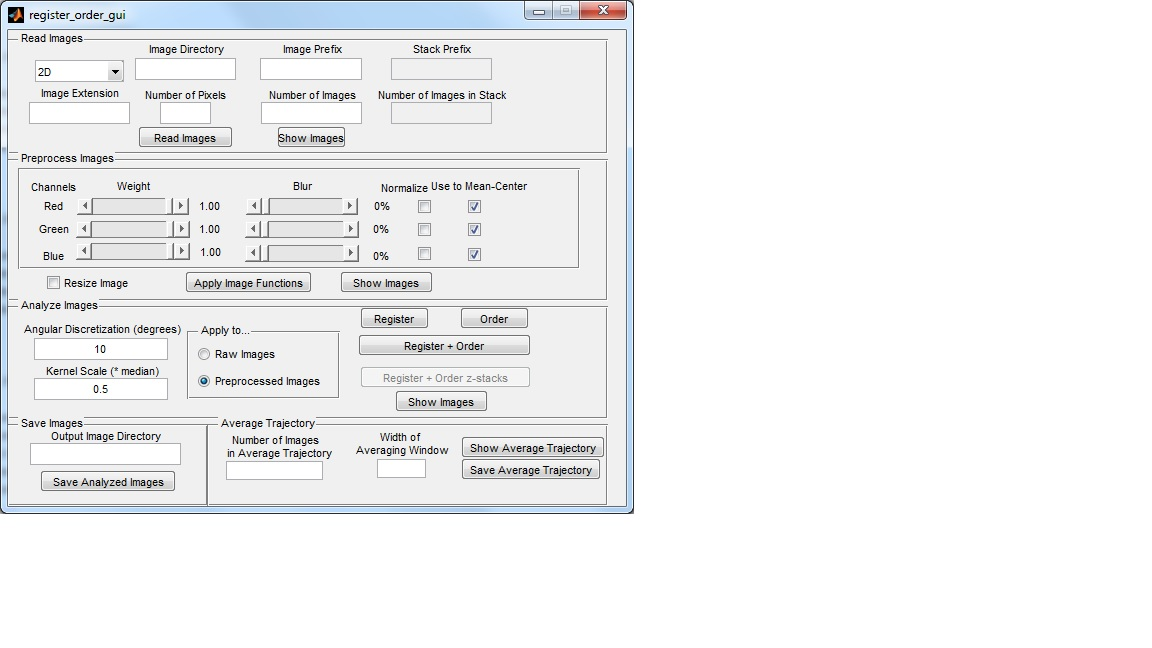
\includegraphics[width=\textwidth, trim=0cm 3cm 12cm 0cm, clip]{gui_screenshot_initial.jpg}


\subsubsection{Read Images}

First populate the relevant parameters for where the images are stored.
%
The fields are as follows
\begin{description}
%
\item[2D/3D] Select ``2D'' if the images are traditional 2D images. Select ``3D'' if the images are z-stacks.
%
\item[Image Directory] Enter the directory where the images or z-stacks are stored. This directory can be an absolute path (e.g. \texttt{C:/Documents/Images}) or a path relative to the directory where this code is stored (e.g. \texttt{../Images})
%
\item[Image Prefix] The prefix for all image file names. The images are assumed to named as the image prefix, followed by a number. 
%
\item[Stack Prefix] (only for 3D z-stacks) The prefix for all stack folder names. Each stack is assumed to be stored in a single folder, with the folder's name as the stack prefix, followed by a number. 
%
\item[Image Extension] The extension of the images (e.g., tif, jpg)
%
\item[Number of Images] The number of images or z-stacks. Images are assumed to be stored as the image prefix, followed by a two-digit index, where the indices run from 1 to the number of images (e.g., image\_prefix01.tif, image\_prefix02.tif, etc.). For three-dimensional images, the z-stacks are assumed to be stored in individual folders whose names are the stack prefix, followed by a two-digit index, where the indices run from 1 to the number of stacks (e.g., z\_stack\_prefix01/, z\_stack\_prefix02/, etc.)
%
\item[Number of Images in Stack] (only for z-stacks) The number of images per z-stack. Images are assumed to be stored in the individual stack directories as the stack prefix, followed by a two-digit index, where the indices run from 1 to the number of images in the stack (e.g., stack\_prefix01.tif, stack\_prefix02.tif, etc.). 
%
\end{description}

After populating the required fields, select the ``Read Images'' button to read in the images.
%
After reading the images, (optional) select the ``Show Images'' button to display the images (z-stacks will be displayed as maximum intensity projections).

\subsubsection{Preprocess Images}

Define the relevant preprocessing operations. 
%
The options are as follows
%
\begin{description}
\item[Weight] Each channel in the images is scaled by the weight factor, where all weights at 1 does not adjust the channel intensities. For grayscale images, only the first weight is used. 
%
\item[Blur] Each channel in the images is blurred using a disc factor with radius equal to a fraction of the image as indicated by the ``blur'' field. For example, setting the blur to 5\% means that the image is blurred using a disc filter with radius $0.05 \times$ the number of pixels. 
%
\item[Normalize] If the normalize option is selected for a specific channel, then Contrast-Limited Adaptive Histogram Equalization is applied to that channel to normalize the intensities across the image. This is important for signals whose absolute intensity is not meaningful or informative. 
%
\item[Use to Mean-Center] If the mean-center option is selected for any of the channels, then the object is centered in the image by detecting the edges of the object given by the selected channels. If no mean-center options are selected, then the object is not mean-centered.
%
\item[Resize Images] If the resize images option is selected, then each image is scaled/dialated so that the object occupies 80\% of the total image frame. This removes any size effects/variations in the images. 
%
\item[Number of Pixels] The number of pixels wanted in the images for analysis. This does {\em not} have to be the same number of pixels as the true resolution of the images. The images are assumed to be square. 
%
\end{description}

After populating the required fields, select the ``Apply Image'' button to apply the selected preprocessing options.
%
After preprocessing the images, (optional) select the ``Show Images'' button to display the preprocessed images (z-stacks will be displayed as maximum intensity projections).

\subsubsection{Analyze Images}

After preprocessing the images, one can apply various analysis algorithms. 
%
There are three parameters
%
\begin{description}
%
\item[Angular Discretization (degrees)] (required for image registration) This is the angular discretization used to search for the pairwise alignments between images. For example, if the angular discretization is 10$^\circ$, then the pairwise alignments are computed by computing the image discrepancy after 10$^\circ$ rotation, after a 20$^\circ$ rotation, ..., up to a 360$^\circ$ rotation, and then selecting the rotation which minimizes the discrepancy. Lower values of the angular discretization increase the accuracy of the method, but also increase the computational cost. 
%
\item[Kernel Scale (*median)] This is the scaling of the diffusion maps kernel, in multiples of the median of the pairwise distances (so that $\epsilon$ in the diffusion maps algorithm, as outlined in \SI, is this value times the median of the pairwise distances). This parameter should be $\mathcal{O}(1)$; empirically, we have found that values of $0.25-0.5$ often yield good results for our data sets. 
%
\item[Apply to...]  This determines which images are shown and/or saved as the analyzed images. Select the ``Apply to Raw Images'' option to apply the computed registration and/or ordering to the original images; select the ``Apply to Preprocessed Images'' option to apply the computed registration and/or ordering to the preprocessed images (after blurring, normalization, etc.)
%
\end{description}

There are four analysis options
\begin{description}
%
\item[Register] (this option is only for two-dimensional images) This registers the imaging data set using vector diffusion maps to compute the optimal rotations. 
%
\item[Order] This orders the imaging data set using diffusion maps. {\em Important:} This option assumes that the imaging data set is preregistered! This option is intended for imaging data sets that were preregistered using some {\em a priori} knowledge about the system. 
%
\item[Register + Order] (this option is only for two-dimensional images) This registers and orders the imaging data set using vector diffusion maps to compute the optimal rotations and the temporal ordering. 
%
\item[Register + Order z-stacks] (this option is only for three-dimensional z-stacks) This registers and orders the imaging data set. It first registers the z-stacks by computing the optimal rotations to align the (two-dimensional) maximum intensity projections along the z-axis using angular synchronization. It then orders the data using diffusion maps on the (now registered) three-dimensional z-stacks. 
%
\end{description}

(Optional) After analysis select the ``Show Images'' button to display the registered and/or images (z-stacks will be displayed as maximum intensity projections). 


\subsubsection{Save Images}

This is the (optional) step of saving the analyzed images.
%
The ``Output Image Directory'' is where the analyzed images will be stored; this directory will be created if it does not exist. 
%
The images will be stored in the output directory, and the name format will be the same as in the input directory. 

\subsubsection{Average Trajectory}

An (optional) step is to compute the average trajectory of the registered and ordered images.

There are two parameters
\begin{description}
\item[Number of Images in Average Trajectory] This is the desired number of images in the average trajectory. 
%
\item[Width of Averaging Window] This is the (approximate) width of the averaging window. Each snapshot in the average trajectory will be the (weighted) average of approximately the width number of images (see \SI). Increasing this value will result in a smoother average trajectory, while decreasing this value will retain more finer-scale detail. 
% 
\end{description}

The ``Show Average Trajectory'' option will then display the average trajectory images. 
%
The ``Save Average Trajectory'' option will save the average trajectory images. 
%
The images will be saved in the ''Output Image Directory'' folder. 
%
The name format will be the same as the input file format, but with the prefix ``avg\_''.

\subsection{Script}

First, make sure that the directory which stores the downloaded code is on your MATLAB path, or that you are in that directory in MATLAB. 

\subsubsection{Read Images}

\begin{par}
The first step is to read in images, using the \texttt{read\_images} function. For two-dimensional images, it requires that all the images are stored in a single directory, all with a consistent prefix, and indexed with two digits starting from \texttt{01}. For three-dimensional z-stack, it assumes each z-stack is stored in a single directory. All of the z-stack directories are required to begin with a consistent prefix, and be indexed with two digits starting from \texttt{01}. Similarly, all of the images are required to begin with a consistent prefix, and be indexed with two digits starting from \texttt{01} for each z-stack.
\end{par} \vspace{1em}
\begin{verbatim}
% directory where images are stored
image_dir = 'drosophila_fixed_images';

% prefix for each image
image_name = 'emb';

% image type/extension
image_ext = 'tif';

% no stack name or number of iamges in a stack are required for 2D images
stack_name = '';
nstack = 0;

% number of images
nimages = 120;

% dimension of images (dim=2 indicates standard 2D images, rather than
% z-stacks)
dim = 2;

% read in images
% images are stored in the variable images_raw
% nchannels stores the number of channels per image
[images_raw, nchannels] = read_images(image_dir, image_name, image_ext, ...
    stack_name, nimages, nstack, dim);
\end{verbatim}


\subsubsection{Show images}

\begin{par}
An optional step is to now show the images using the \texttt{plot\_images} function.
\end{par} \vspace{1em}
\begin{verbatim}
% plot the images
% images_raw are the images to plot
% (returned from the read_images function)
% dim is the dimension of the images
% (dim=2 indicates standard 2D images, rather than z-stacks)
plot_images(images_raw, dim)
\end{verbatim}

\includegraphics [width=4in]{sample_input_file_01.jpg}


\subsubsection{Preprocess Images}

\begin{par}
Now, we must preprocess the images using the \texttt{apply\_image\_functions} function before registration and ordering, to remove any imaging and/or experimental artifacts.
\end{par} \vspace{1em}
\begin{verbatim}
% number of pixels
% images will be reduced to npixels x npixels resolution
npixels = 100;

% channel weights
% we scale the first (red) channel by half, and keep the second (green) and
% third (blue) channels at their input values
channel_weight = [0.5 1 1];

% channel blur
% we blur each of the channels by 5%
channel_blur = [0.05 0.05 0.05];

% channel normalization
% we normalize the first (red) channel using histogram equalization
% we do not normalize the second (green) or third (blue) channels
channel_normalize = [1 0 0];

% mean-center
% we use the first (red) channel to detect the edges of the object in order
% to mean center the object
channel_mean_center = [1 0 0];

% resize
% we choose to resize the images so all objects are (approximately)
% the same size, to remove any variations due to size effects
resize_image = true;

% we then apply these image functions of normalization, blurring,
% reweighting, and mean-centering
images = apply_image_functions(images_raw, npixels, dim, channel_weight, ...
    channel_blur, channel_normalize, channel_mean_center, resize_image);

% plot the images (optional)
plot_images(images, dim)
\end{verbatim}

\includegraphics [width=4in]{sample_input_file_02.jpg}


\subsubsection{Calculate pairwise alignments}

\begin{par}
We now need to calculate the angles needed to align \textit{pairs} of images
\end{par} \vspace{1em}
\begin{verbatim}
% angular discretization when computing pairwise aligments
% this means we search for pairwise aligmemnts over 10 degree increments
ang_dis = 10;

% compute the pairwise alignments
% images are the preprocessed images
% ang_dis is the angular discretization
% R and W store the pairwise alignments and distances, respectively, for
% vector diffusion maps
[R, W] = compute_pairwise_alignments(images, ang_dis);
\end{verbatim}


\subsubsection{Apply vector diffusion maps}

\begin{par}
We can now use vector diffusion maps to register and order the images.
\end{par} \vspace{1em}
\begin{verbatim}
% ncomps is the number of components to compute
% we only compute 1 coordinate because we only need to order the images
% (i.e., sort by the first coordinate)
ncomps = 1;

% epsilon scale for diffusion maps kernel
% eps_scale = 0.25 means that the epsilon in the diffusion maps kernel is
% 1/4 of the median of the pairwise distances between data points
eps_scale = 0.25;

% vector diffusion maps calculates optimal rotations and embedding
% coordinate
[R_opt, embed_coord, D2] = vdm(R, W, eps_scale, ncomps);

% register images
images_registered = register_all_images(images, R_opt);

% order registered images by embedding coordinate
images_analyzed = order_all_images(images_registered, embed_coord);

% plot the images (optional)
plot_images(images_analyzed, dim)
\end{verbatim}

\includegraphics [width=4in]{sample_input_file_03.jpg}

\subsubsection{Calculate average trajectory}

\begin{par}
We can calculate an average trajectory from our set of (registered and ordered) images
\end{par} \vspace{1em}
\begin{verbatim}
% nsubimages is the desired number of images in the average trajectory
nsubimages = 10;

% avg_width is the (approximate) width of the averaging window used to
% compute each of the images in the average trajectory
avg_width = 4;

% compute the average trajectory
avg_images = compute_average_trajectory(images_analyzed, nsubimages, avg_width);

% plot the images (optional)
plot_images(avg_images, dim)
\end{verbatim}

\includegraphics [width=4in]{sample_input_file_04.jpg}

\section{Parameters for Data Sets}

The four data sets used in the paper are available with the code in the relevant subdirectories. The parameters used (as defined in the script in the previous section) are defined below. 

\subsection{{\em Drosophila} gastrulation (live)}

\begin{verbatim}

image_dir = 'drosophila_live_imaging/expt01';
image_name = 'image';
image_ext = 'tif';
stack_name = '';
nimages = 40;
nstack = 0;
dim = 2;

npixels = 100;
channel_weight = 1;
channel_blur = 0.05;
channel_normalize = 1;
channel_mean_center = 0;
resize_image = false;

ang_dis = 10;

eps_scale = 0.25;

\end{verbatim}


\subsection{Zebrafish epiboly}

\begin{verbatim}

image_dir = 'zebrafish';
image_name = 'image';
image_ext = 'tif';
stack_name = '';
nimages = 120;
nstack = 0;
dim = 2;

npixels = 100;
channel_weight = 1;
channel_blur = 0;
channel_normalize = 0;
channel_mean_center = 1;
resize_image = false;

ang_dis = 10;

eps_scale = 0.25;

\end{verbatim}


\subsection{{\em Drosophila} gastrulation (fixed)}

\begin{verbatim}

image_dir = 'drosophila_fixed_images';
image_name = 'emb';
image_ext = 'tif';
stack_name = '';
nimages = 120;
nstack = 0;
dim = 2;

npixels = 100;
channel_weight = [0.5 1 1];
channel_blur = [0.05 0.05 0.05];
channel_normalize = [1 0 0];
channel_mean_center = [1 0 0];
resize_image = true;

ang_dis = 10;

eps_scale = 0.25;

\end{verbatim}


\subsection{{\em Drosophila} wing discs}

\begin{verbatim}

image_dir = 'wing_disc_stacks';
image_name = 'disc';
image_ext = 'tif';
stack_name = 'z';
nimages = 46;
nstack = 21;
dim = 3;

npixels = 100;
channel_weight = [1 1 1];
channel_blur = [0 0 0];
channel_normalize = [0 0 0];
channel_mean_center = [0 0 1];
resize_image = false;

ang_dis = 10;

eps_scale = 0.5;
\end{verbatim}

\section{Parameter Values and Guidance}

\begin{description}

\item[Weight] The relative weights of the channels in multichannel images in important for computing meaningful distances for diffusion maps. The total intensity for each channel should be of the same order if all channels are to be considered as ``equally important.'' If the channels have dramatically different intensities in the raw images, they should be adjusted via the weight functions.
%
\item[Blur] The image should be blurred to remove fine-scale noise and variations. Typically, blur of 5\%-10\% are appropriate for removing such variability. In some cases, blurring is not necessary to recover an accurate registration and ordering. 
%
\item[Normalize] Channels should be normalized if the absolute intensity of a specific signal is not meaningful. For example, DAPI, a DNA marker, identifies the nuclei in the {\em Drosophila} embryo, but the absolute intensity of the signal is not important. 
%
\item[Use to Mean-Center] Objects should be (approximately) mean-centered in the frame prior to registration. The channel(s) that best identify/delineate the periphery of the object should be selected for use in the mean-centering procedure.
%
\item[Resize Images] Object should be resized if size differences are not meaningful/informative about the underlying developmental dynamics. 
%
\item[Number of Pixels] The image resolution should be chosen as low as possible such that the relevant developmental structures and patterns are still discernible/evident. A higher image resolution will result in a higher computational cost. 
%
\item[Kernel Scale] The kernel scale defines how similar two images have to be to be considered developmentally close. Small values of the kernel will preserve finer scale patternds and structure in the ordering algorihtm, but will also be more sensitive to noise. We have found values of 0.25-0.5 to often be suitable for our studies. Noisy data with a lower temporal resolution (such as the wing disc data) often requires a larger value of the kernel scale than clean data with a high temporal resolution (such as the zebrafish live imaging data). 
%
\item[Angular Discretization] The angular discretization sets the resolution for computing the pairwise alignments. For example, if the angular discretization is 10$^\circ$, then the pairwise alignments are computed by computing the image discrepancy after 10$^\circ$ rotation, after a 20$^\circ$ rotation, ..., up to a 360$^\circ$ rotation, and then selecting the rotation which minimizes the discrepancy. Lower values of the angular discretization increase the accuracy of the method, but also increase the computational cost. We have found that $10^\circ$ is often a good value of the angular discretization, which balances computational cost and accuracy.

\end{description}

\end{document}

